\documentclass[11pt,a4paper]{article}
\usepackage[margin=0.75in]{geometry}
\usepackage{hyperref}
\usepackage{pdfpages}
\usepackage{bookmark}
\usepackage{xcolor}

% Enhanced hyperlink setup
\hypersetup{
    colorlinks=true,
    linkcolor=blue,
    urlcolor=blue,
    bookmarks=true,
    bookmarksopen=true,
    bookmarksnumbered=true,
    pdfstartview=FitH,
    pdftitle={NMAMIT Complete Examination Question Bank - Unified},
    pdfauthor={NMAM Institute of Technology},
    pdfsubject={IV Semester B.E./B.Tech Question Papers 2022-2025}
}

\begin{document}

% ========== UNIFIED TITLE PAGE WITH CLICKABLE MENU ==========
\begin{titlepage}
\centering
\vspace*{1.5cm}
{\Huge\bfseries NMAM Institute of Technology, Nitte\par}
\vspace{0.5cm}
{\Large\itshape Off-Campus Centre of Nitte (Deemed to be University)\par}
\vspace{2cm}
{\Huge\bfseries COMPLETE EXAMINATION\\QUESTION BANK\par}
\vspace{0.5cm}
{\large\bfseries Unified Edition with Single Navigation Menu\par}
\vspace{1cm}
{\Large IV Semester B.E./B.Tech (CBCS)\par}
\vspace{0.5cm}
{\Large Academic Years: 2022--2025\par}
\vspace{1.5cm}

{\Large\bfseries\textcolor{blue}{Quick Navigation - Click Any Item:}\par}
\vspace{0.8cm}

\begin{tabular}{|p{3.5cm}|p{8cm}|c|}
\hline
\textbf{Subject Code} & \textbf{Subject Name} & \textbf{Page} \\
\hline
\hyperlink{section.1}{MA2005-1} & \hyperlink{section.1}{Linear Algebra \& Numerical Methods} & \hyperlink{section.1}{4} \\
\hline
\hyperlink{section.2}{CS2102-1} & \hyperlink{section.2}{Database Management Systems} & \hyperlink{section.2}{14} \\
\hline
\hyperlink{section.3}{CS3004-1} & \hyperlink{section.3}{Design and Analysis of Algorithms} & \hyperlink{section.3}{20} \\
\hline
\hyperlink{section.4}{CS2103-1} & \hyperlink{section.4}{Software Engineering \& Project Management} & \hyperlink{section.4}{30} \\
\hline
\hyperlink{section.5}{CS3005-1} & \hyperlink{section.5}{Microprocessor \& Embedded Systems} & \hyperlink{section.5}{35} \\
\hline
\hyperlink{section.6}{ME1654-1} & \hyperlink{section.6}{Innovation and Design Thinking} & \hyperlink{section.6}{40} \\
\hline
\end{tabular}

\vspace{1.5cm}
{\large\bfseries\textcolor{blue}{Additional Resources:}\par}
\vspace{0.5cm}

\begin{itemize}
\item \hyperlink{appendix.A}{Appendix A: Descriptive Questions Collection} (Page 43)
\item \hyperlink{appendix.B}{Appendix B: MCQ Bank} (Page 76)
\item \hyperlink{appendix.C}{Appendix C: Scanned Question Papers} (Page 92)
\item \hyperlink{appendix.D}{Appendix D: Additional MSE Papers} (Page 112)
\end{itemize}

\vspace{1cm}
{\large\textcolor{red}{Tip:} Use PDF bookmarks panel (left sidebar) for detailed navigation\par}

\vfill
{\large Organized by: Subject → MSE-I → MSE-II → SEE\par}
\vspace{0.3cm}
{\small Total: 115 Pages | All Exam Types: MSE-I, MSE-II, SEE (2022-2025)\par}
\end{titlepage}

% ========== DETAILED TABLE OF CONTENTS ==========
\pdfbookmark[0]{Table of Contents}{toc}
\tableofcontents
\newpage

% ========== SECTION 1: LINEAR ALGEBRA ==========
\hypertarget{section.1}{}
\bookmark[dest=section.1,level=0]{LINEAR ALGEBRA AND NUMERICAL METHODS}
\includepdf[pages=4-13,pagecommand={\bookmark[dest=page.\thepage,level=1]{Linear Algebra - MSE \& SEE Papers}}]{COMPLETE_QUESTION_BANK_FROM_LATEX.pdf}

% ========== SECTION 2: DATABASE MANAGEMENT SYSTEMS ==========
\hypertarget{section.2}{}
\bookmark[dest=section.2,level=0]{DATABASE MANAGEMENT SYSTEMS}
\includepdf[pages=14-19,pagecommand={\bookmark[dest=page.\thepage,level=1]{DBMS - MSE \& SEE Papers}}]{COMPLETE_QUESTION_BANK_FROM_LATEX.pdf}

% ========== SECTION 3: DESIGN AND ANALYSIS OF ALGORITHMS ==========
\hypertarget{section.3}{}
\bookmark[dest=section.3,level=0]{DESIGN AND ANALYSIS OF ALGORITHMS}
\includepdf[pages=20-29,pagecommand={\bookmark[dest=page.\thepage,level=1]{DAA - MSE \& SEE Papers}}]{COMPLETE_QUESTION_BANK_FROM_LATEX.pdf}

% ========== SECTION 4: SOFTWARE ENGINEERING ==========
\hypertarget{section.4}{}
\bookmark[dest=section.4,level=0]{SOFTWARE ENGINEERING \& PROJECT MANAGEMENT}
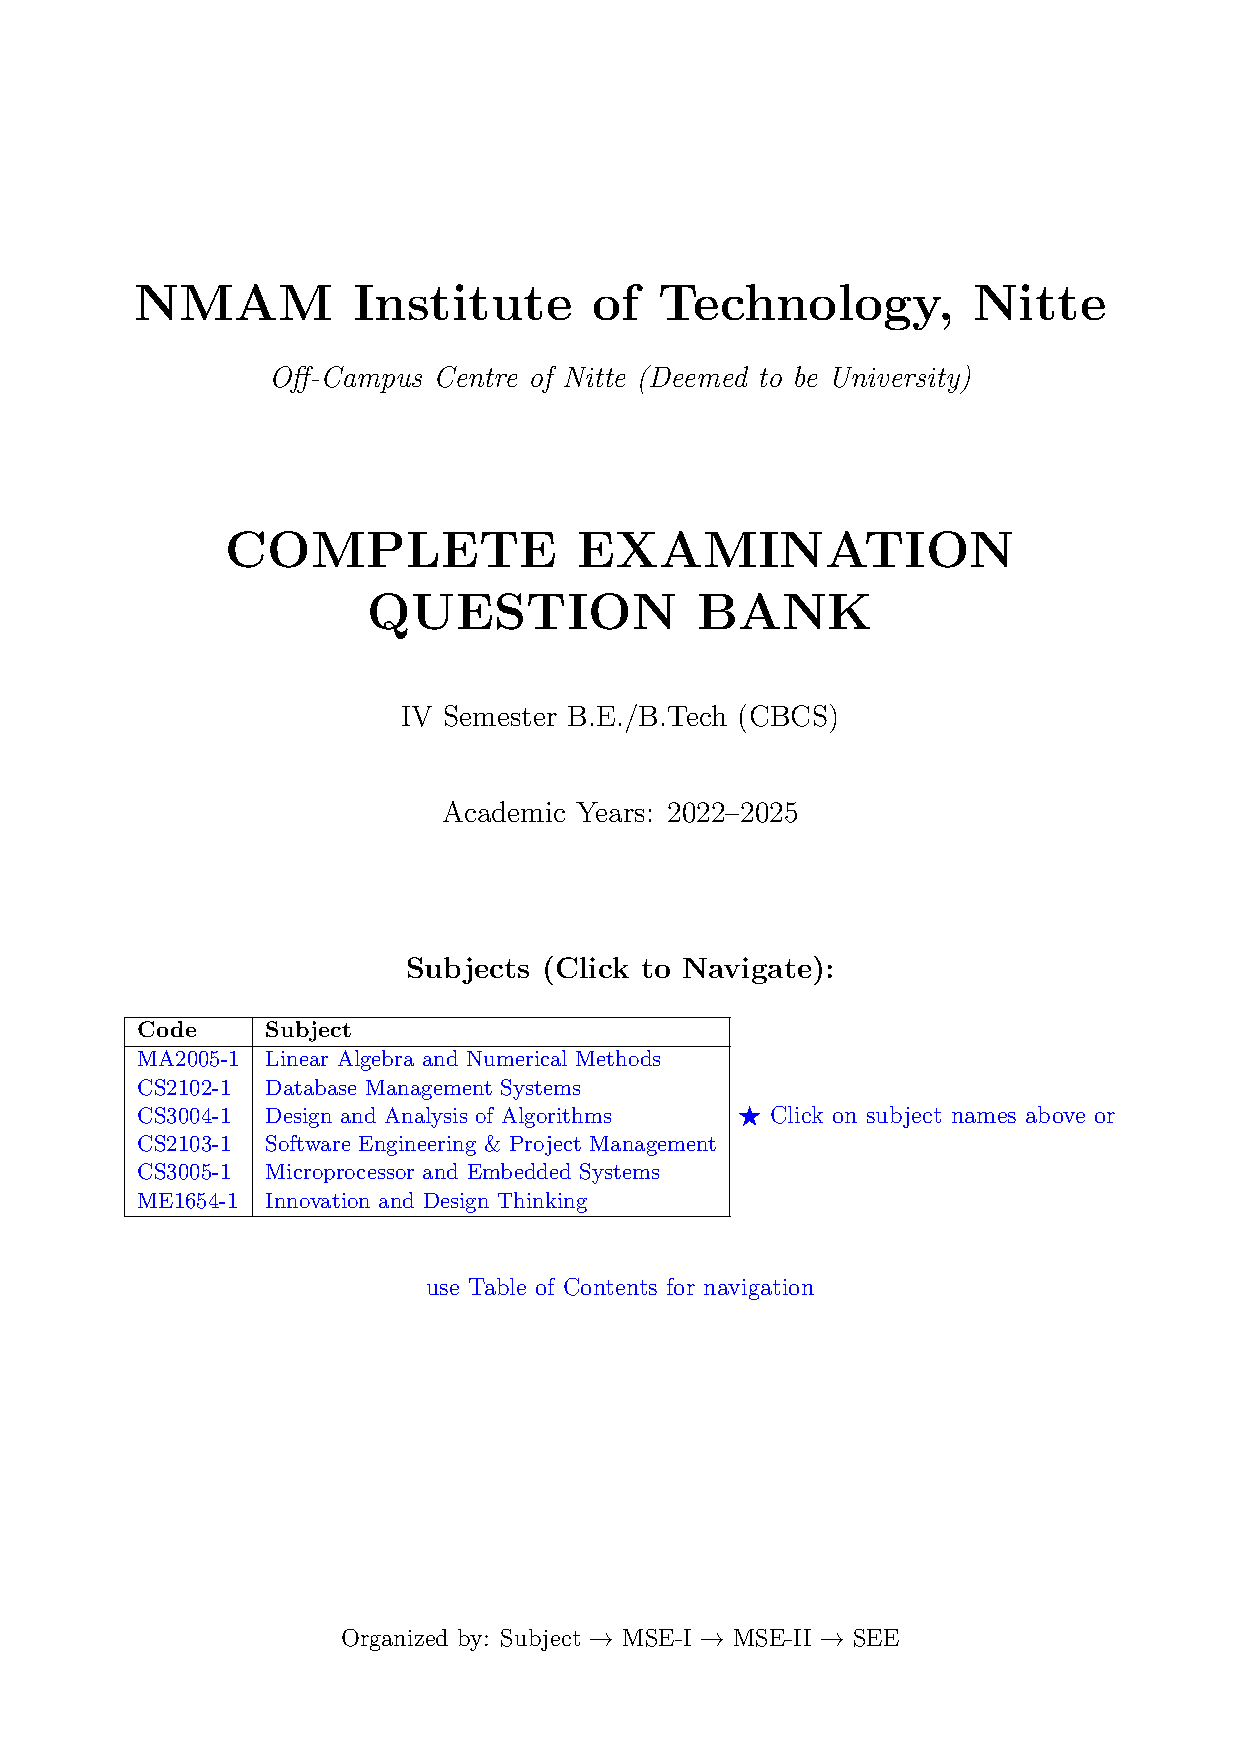
\includepdf[pages=1-5,pagecommand={}]{COMPLETE_QUESTION_BANK_FROM_LATEX.pdf}

% ========== SECTION 5: MICROPROCESSOR ==========
\hypertarget{section.5}{}
\bookmark[dest=section.5,level=0]{MICROPROCESSOR AND EMBEDDED SYSTEMS}
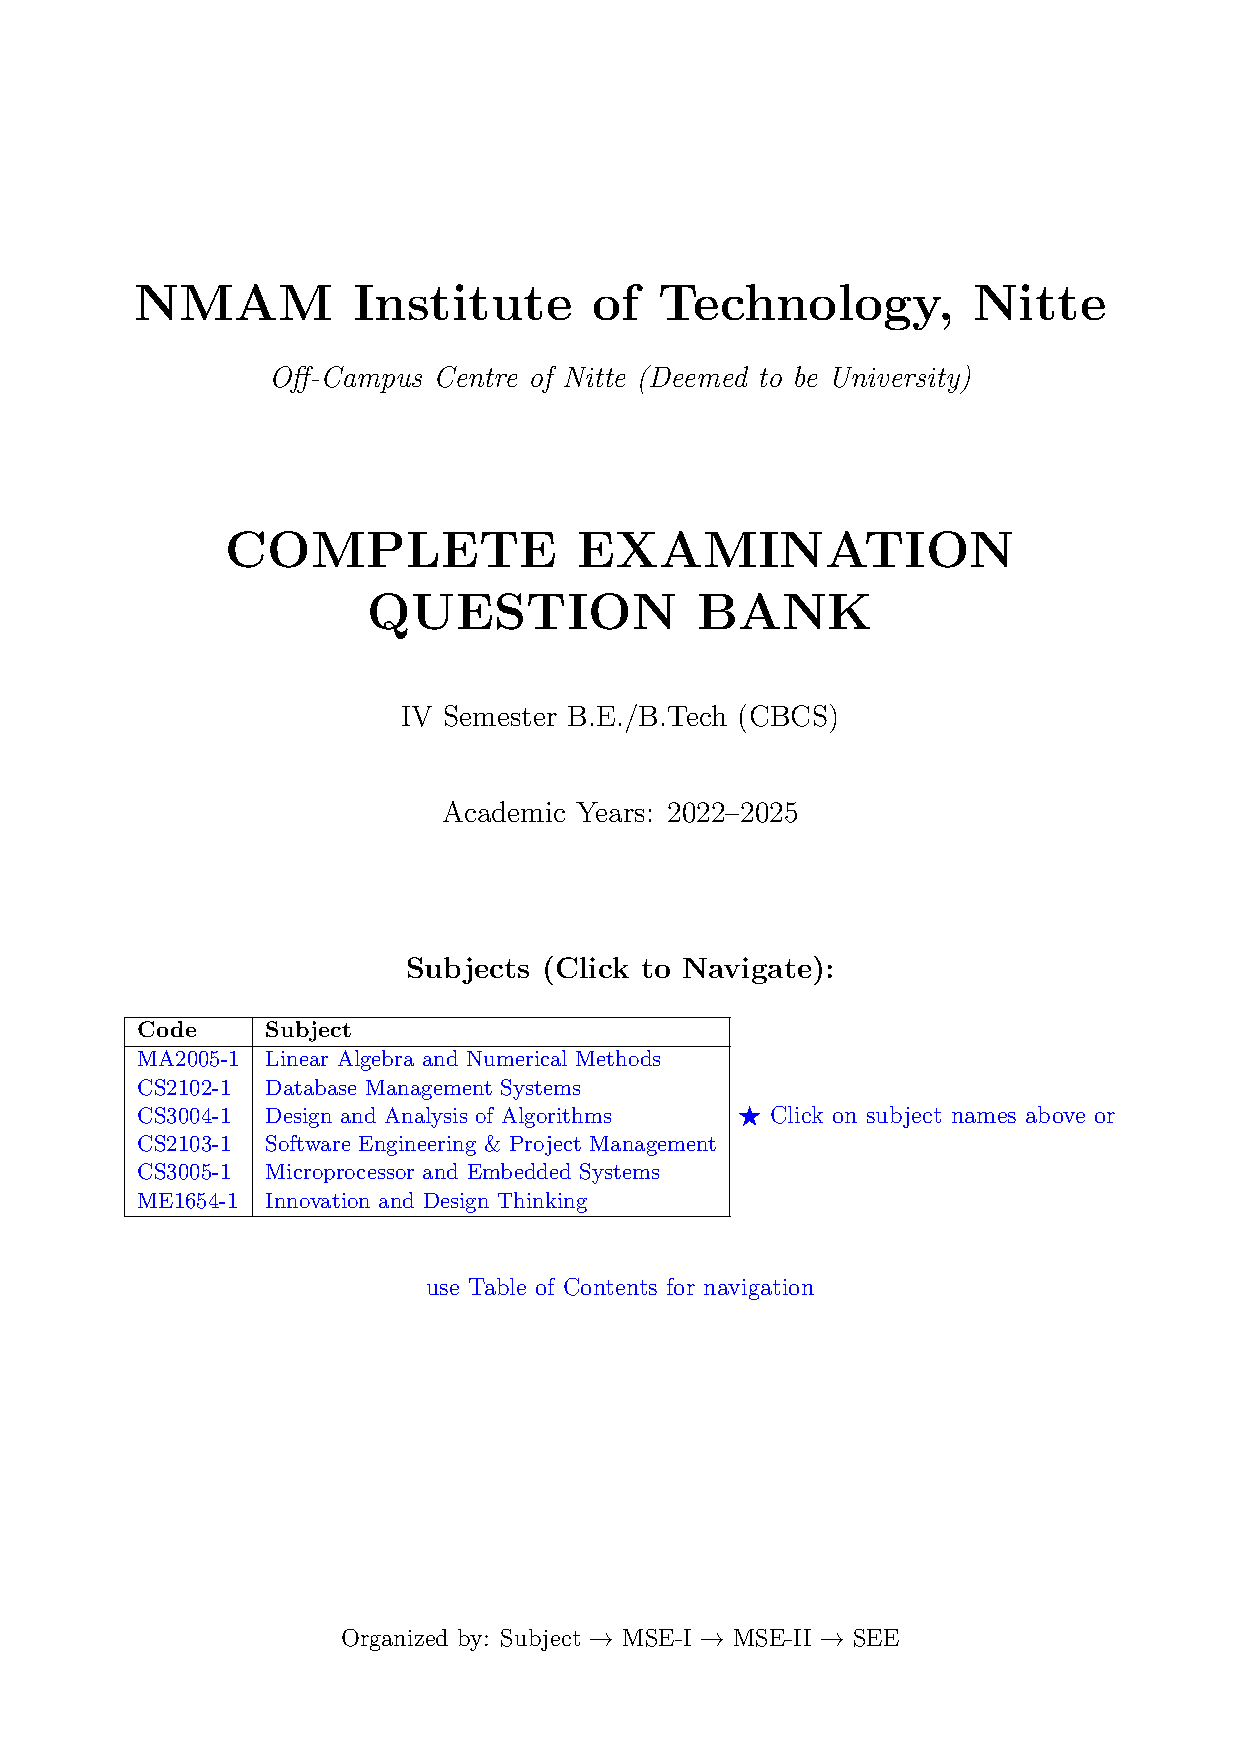
\includepdf[pages=1-5,pagecommand={}]{COMPLETE_QUESTION_BANK_FROM_LATEX.pdf}

% ========== SECTION 6: INNOVATION AND DESIGN THINKING ==========
\hypertarget{section.6}{}
\bookmark[dest=section.6,level=0]{INNOVATION AND DESIGN THINKING}
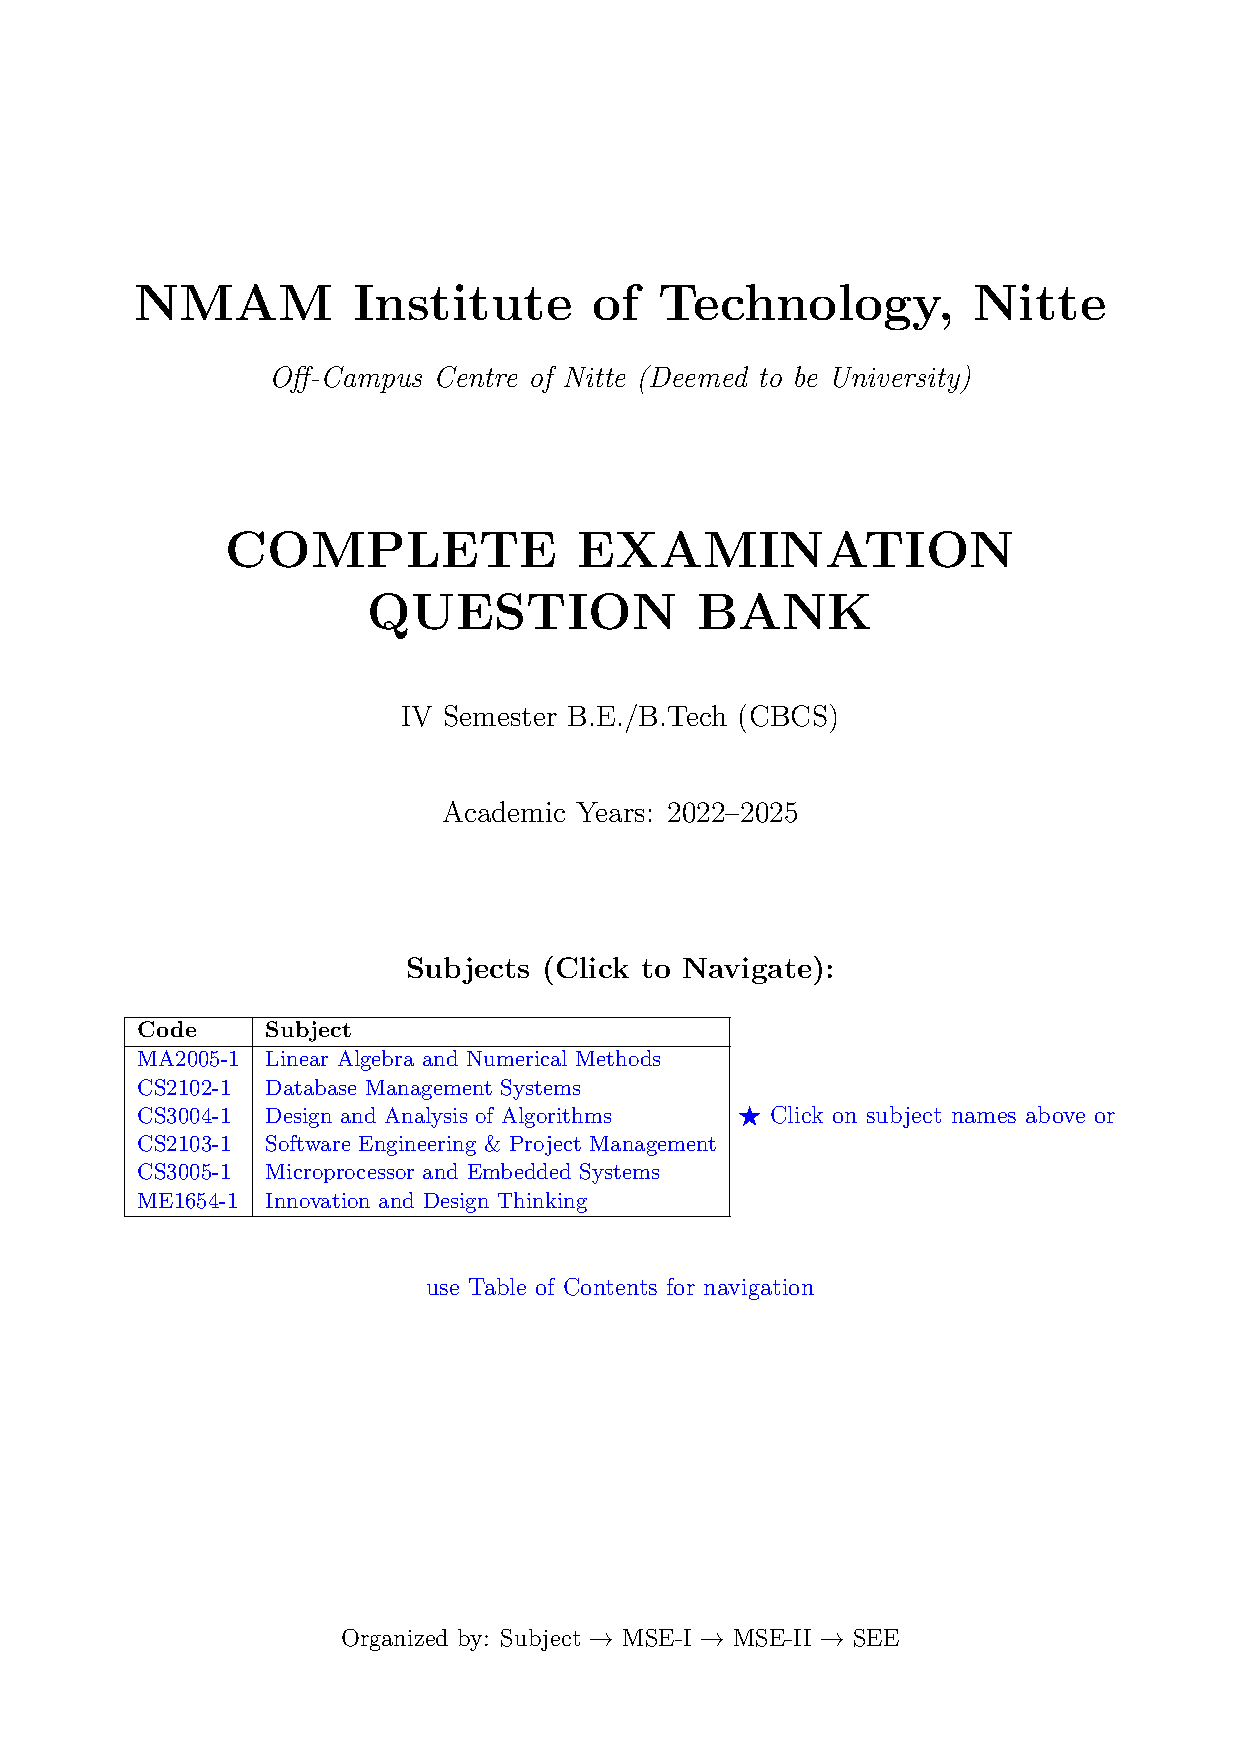
\includepdf[pages=1-3,pagecommand={}]{COMPLETE_QUESTION_BANK_FROM_LATEX.pdf}

% ========== APPENDIX A: SOURCE EXAM BANK ==========
\hypertarget{appendix.A}{}
\bookmark[dest=appendix.A,level=0]{APPENDIX A: Descriptive Questions Collection}
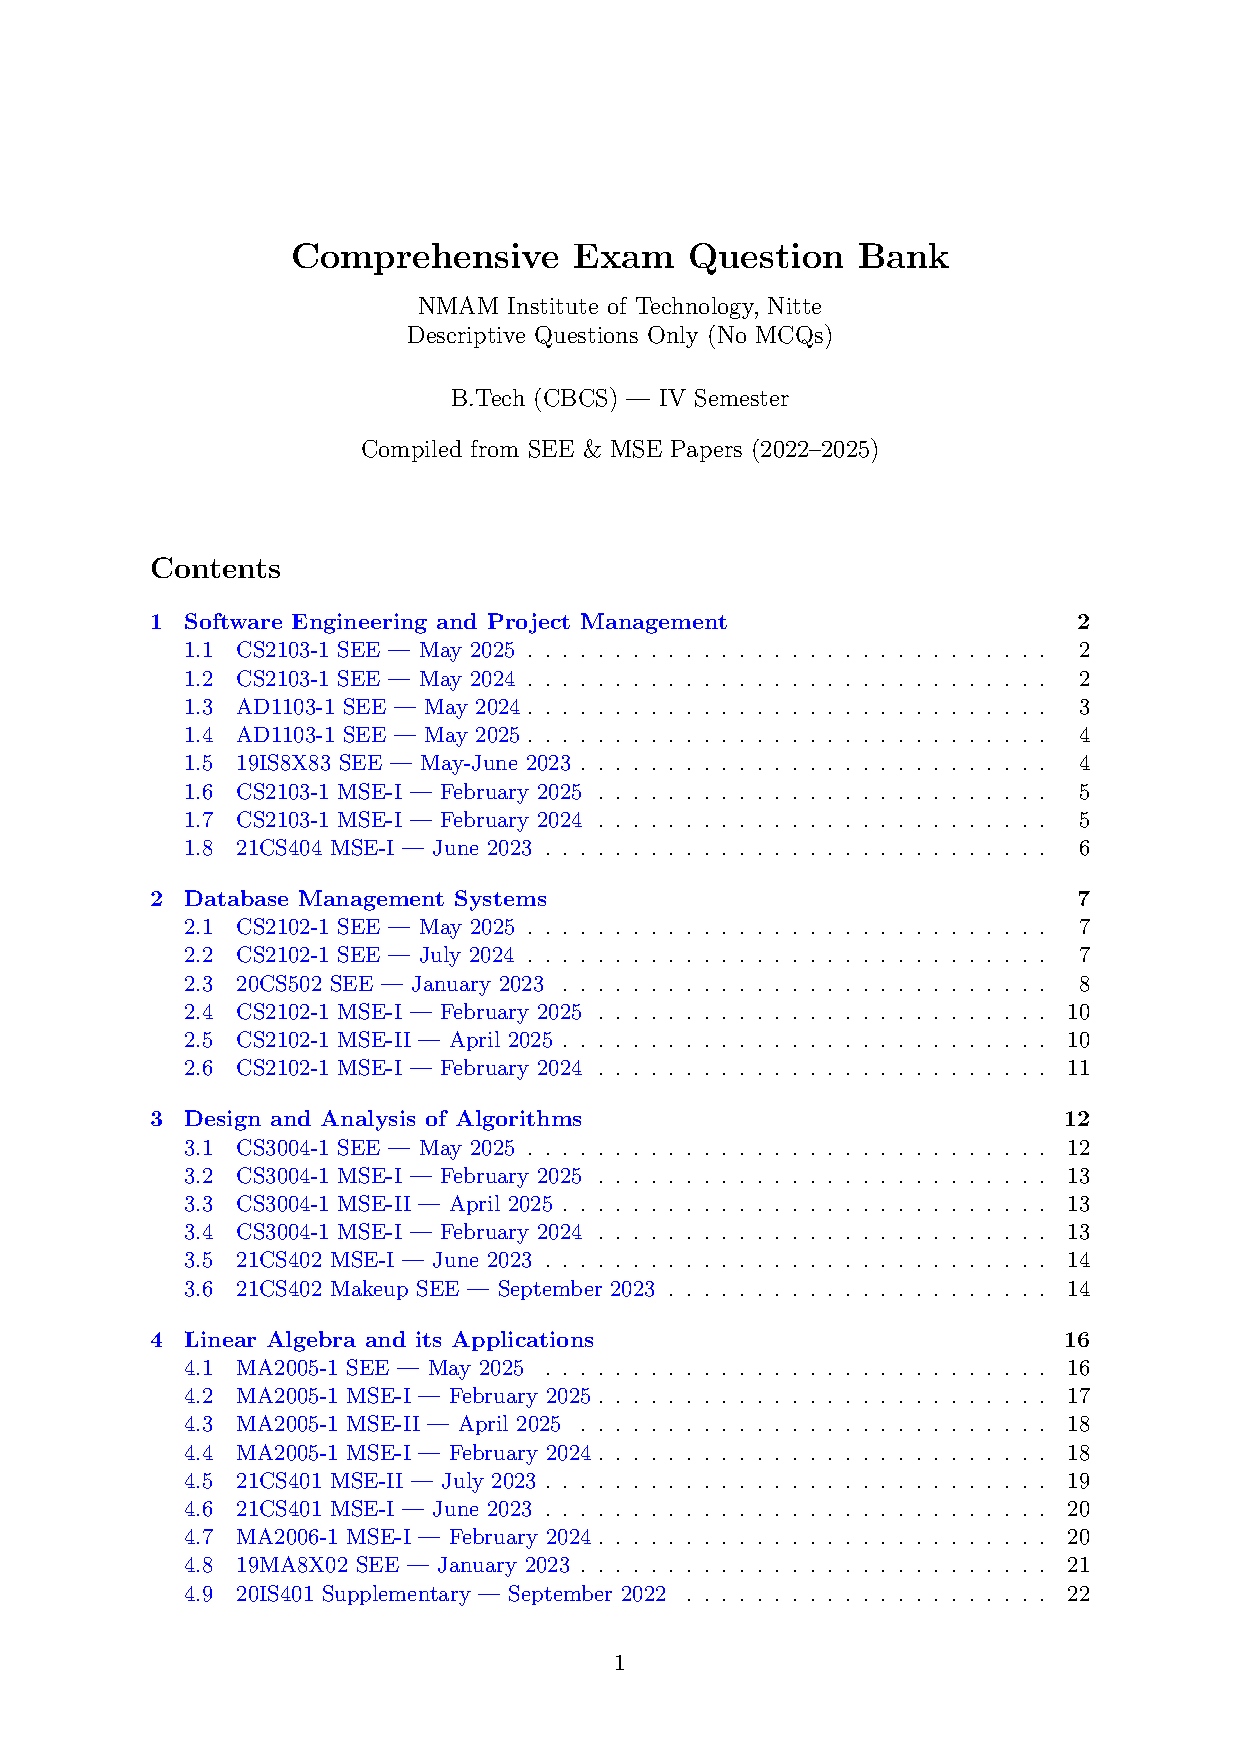
\includepdf[pages=-,pagecommand={\thispagestyle{plain}}]{source_exam_bank.pdf}

% ========== APPENDIX B: EXAM QUESTION BANK ==========
\hypertarget{appendix.B}{}
\bookmark[dest=appendix.B,level=0]{APPENDIX B: MCQ Bank}
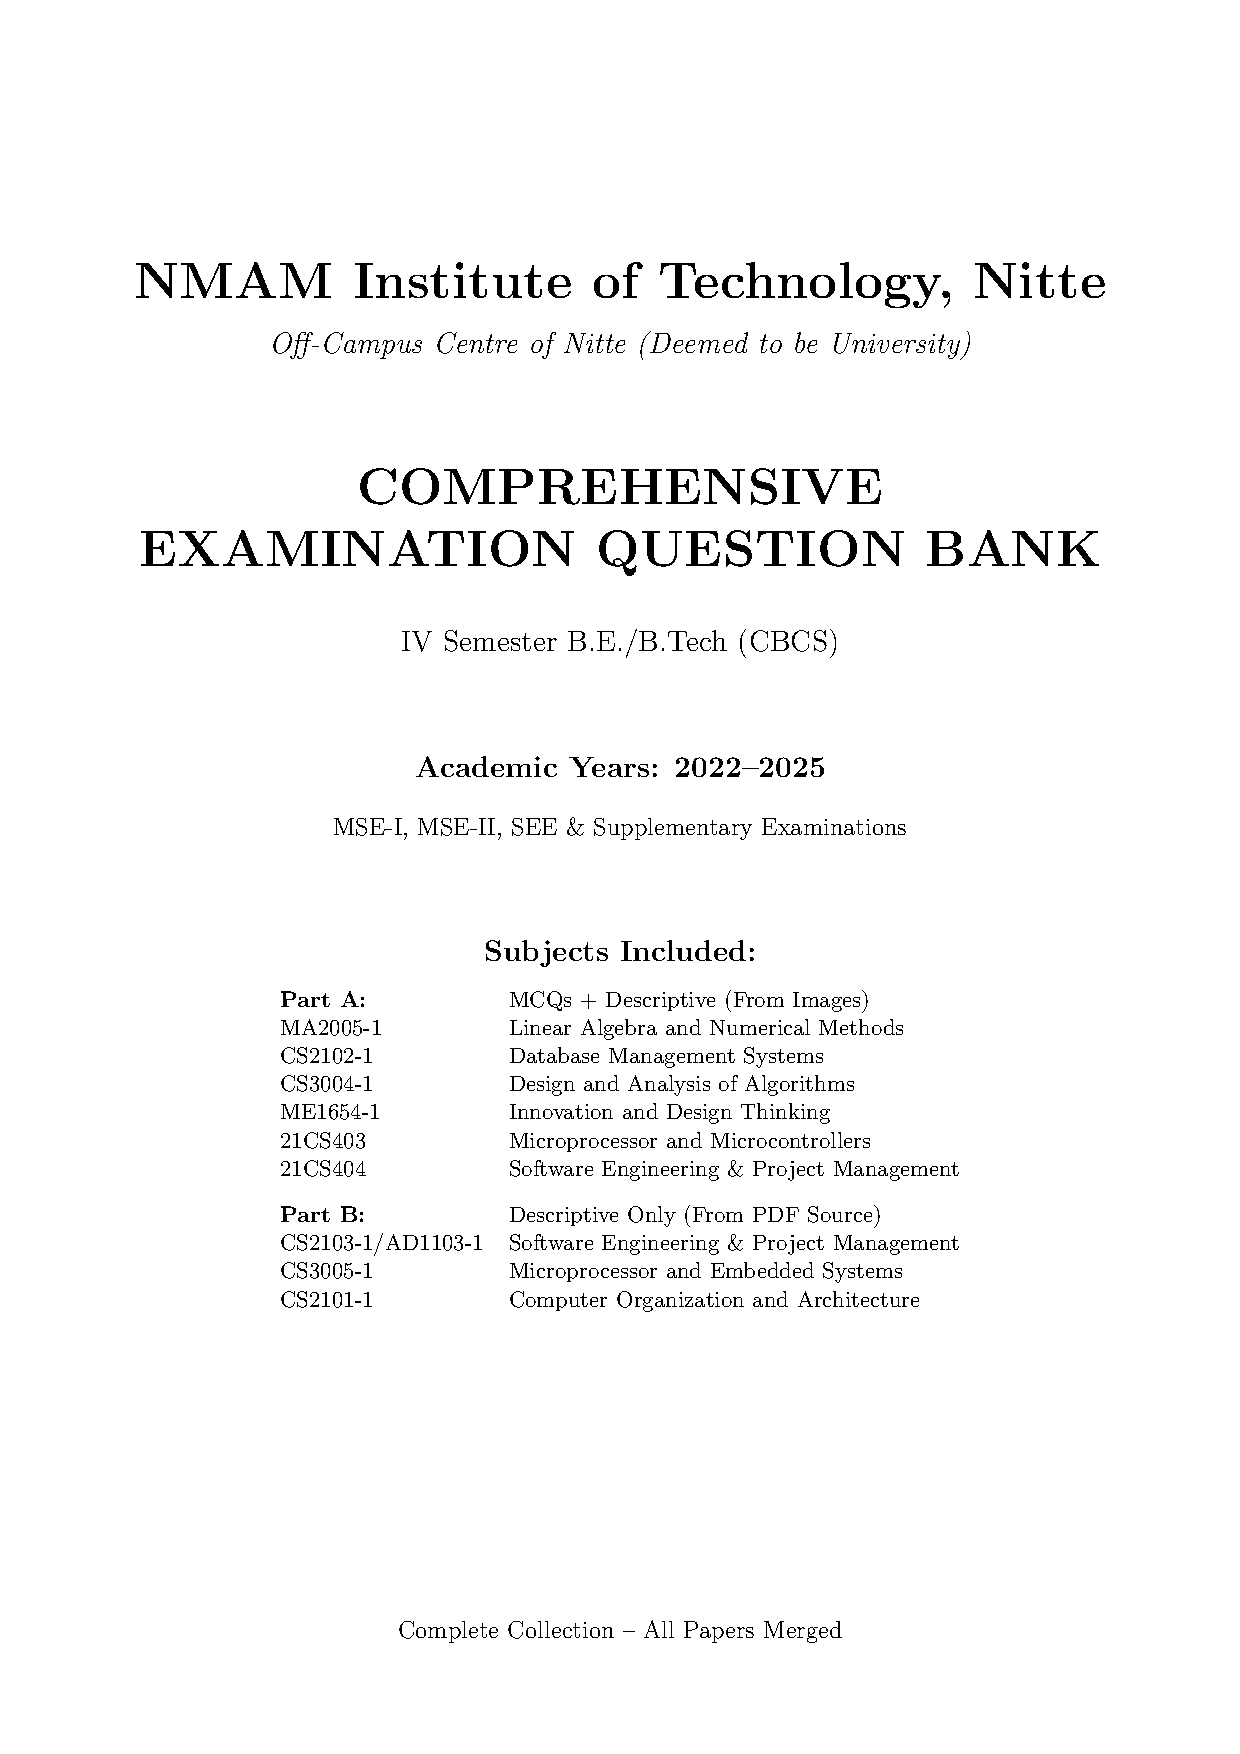
\includepdf[pages=-]{exam_question_bank.pdf}

% ========== APPENDIX C: MSE PAPERS SCANNED ==========
\hypertarget{appendix.C}{}
\bookmark[dest=appendix.C,level=0]{APPENDIX C: Scanned Question Papers}
\includepdf[pages=-]{mse papers.pdf}

% ========== APPENDIX D: ADDITIONAL PAPERS ==========
\hypertarget{appendix.D}{}
\bookmark[dest=appendix.D,level=0]{APPENDIX D: Additional MSE Papers}
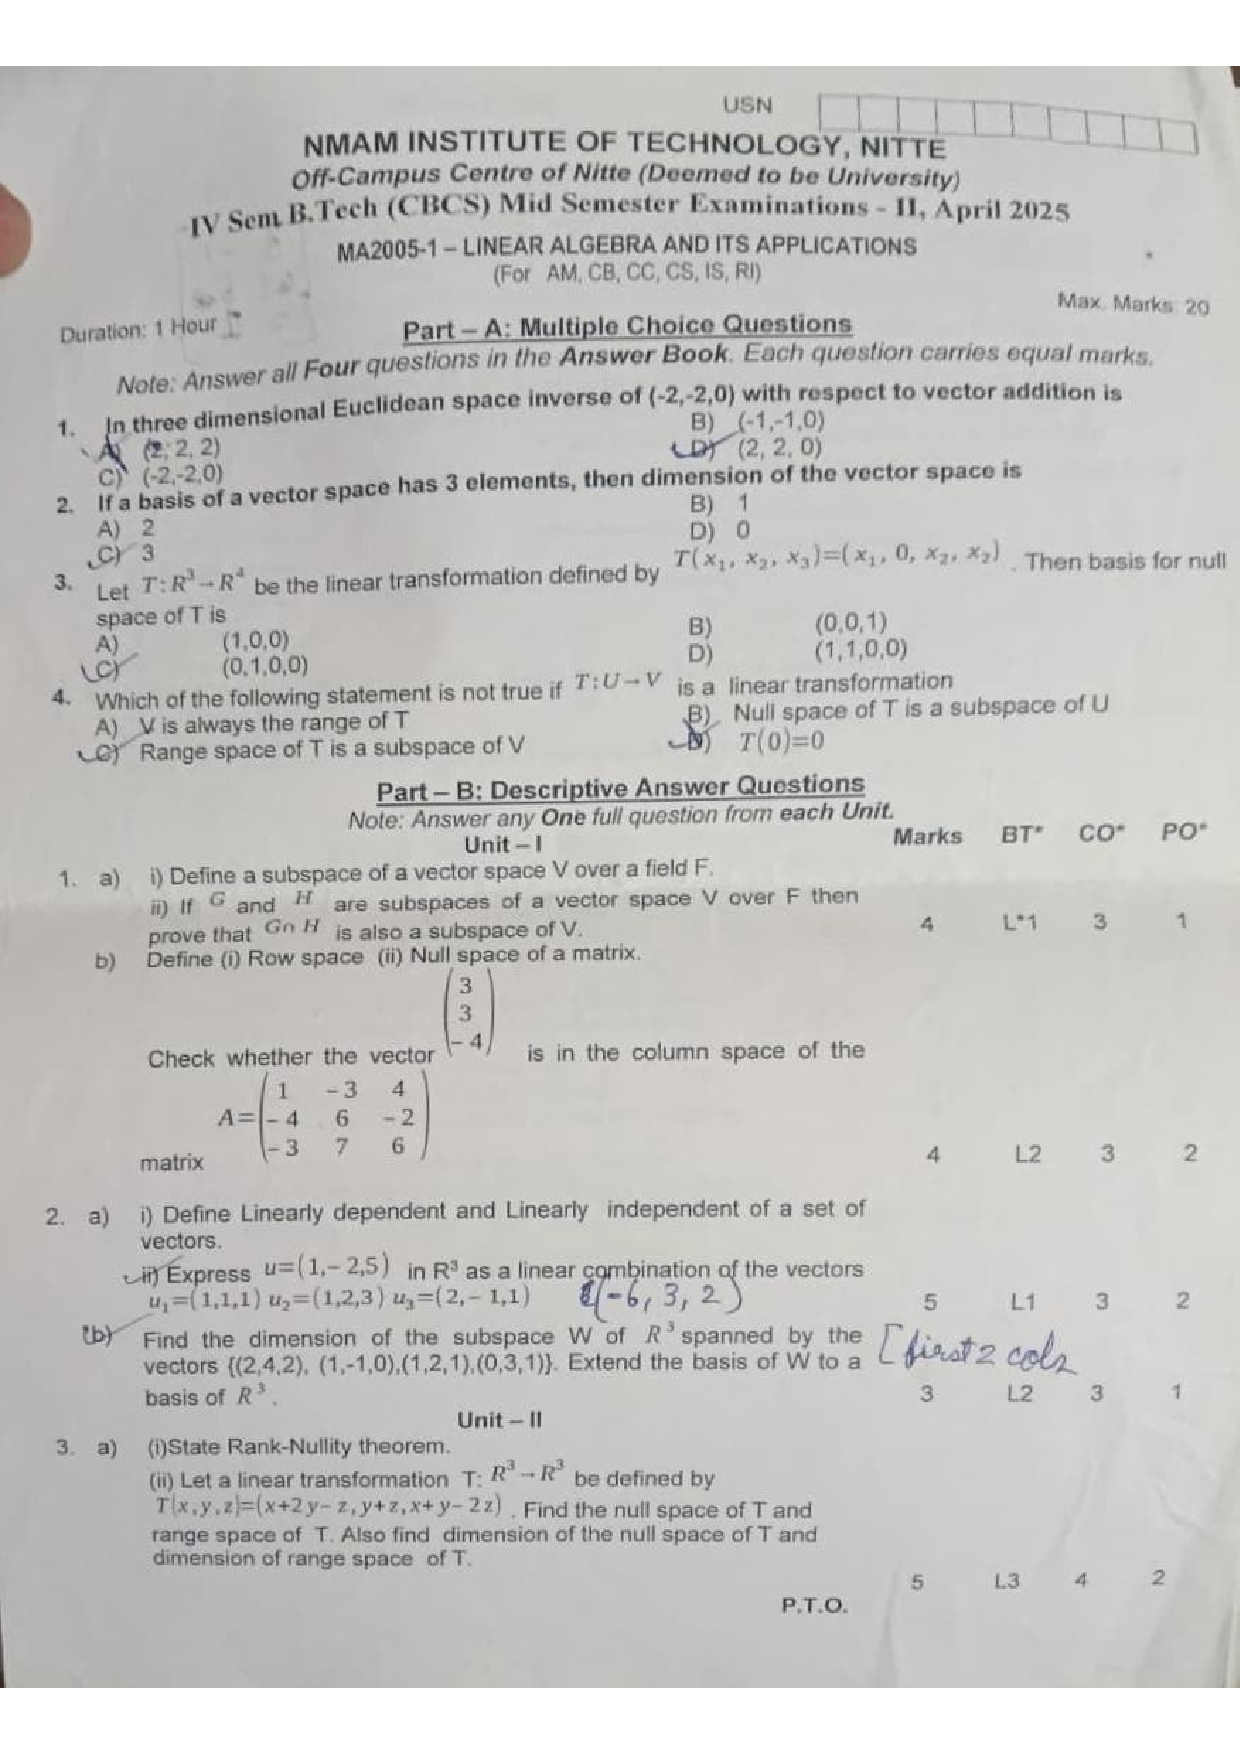
\includepdf[pages=-]{mse2_source.pdf}
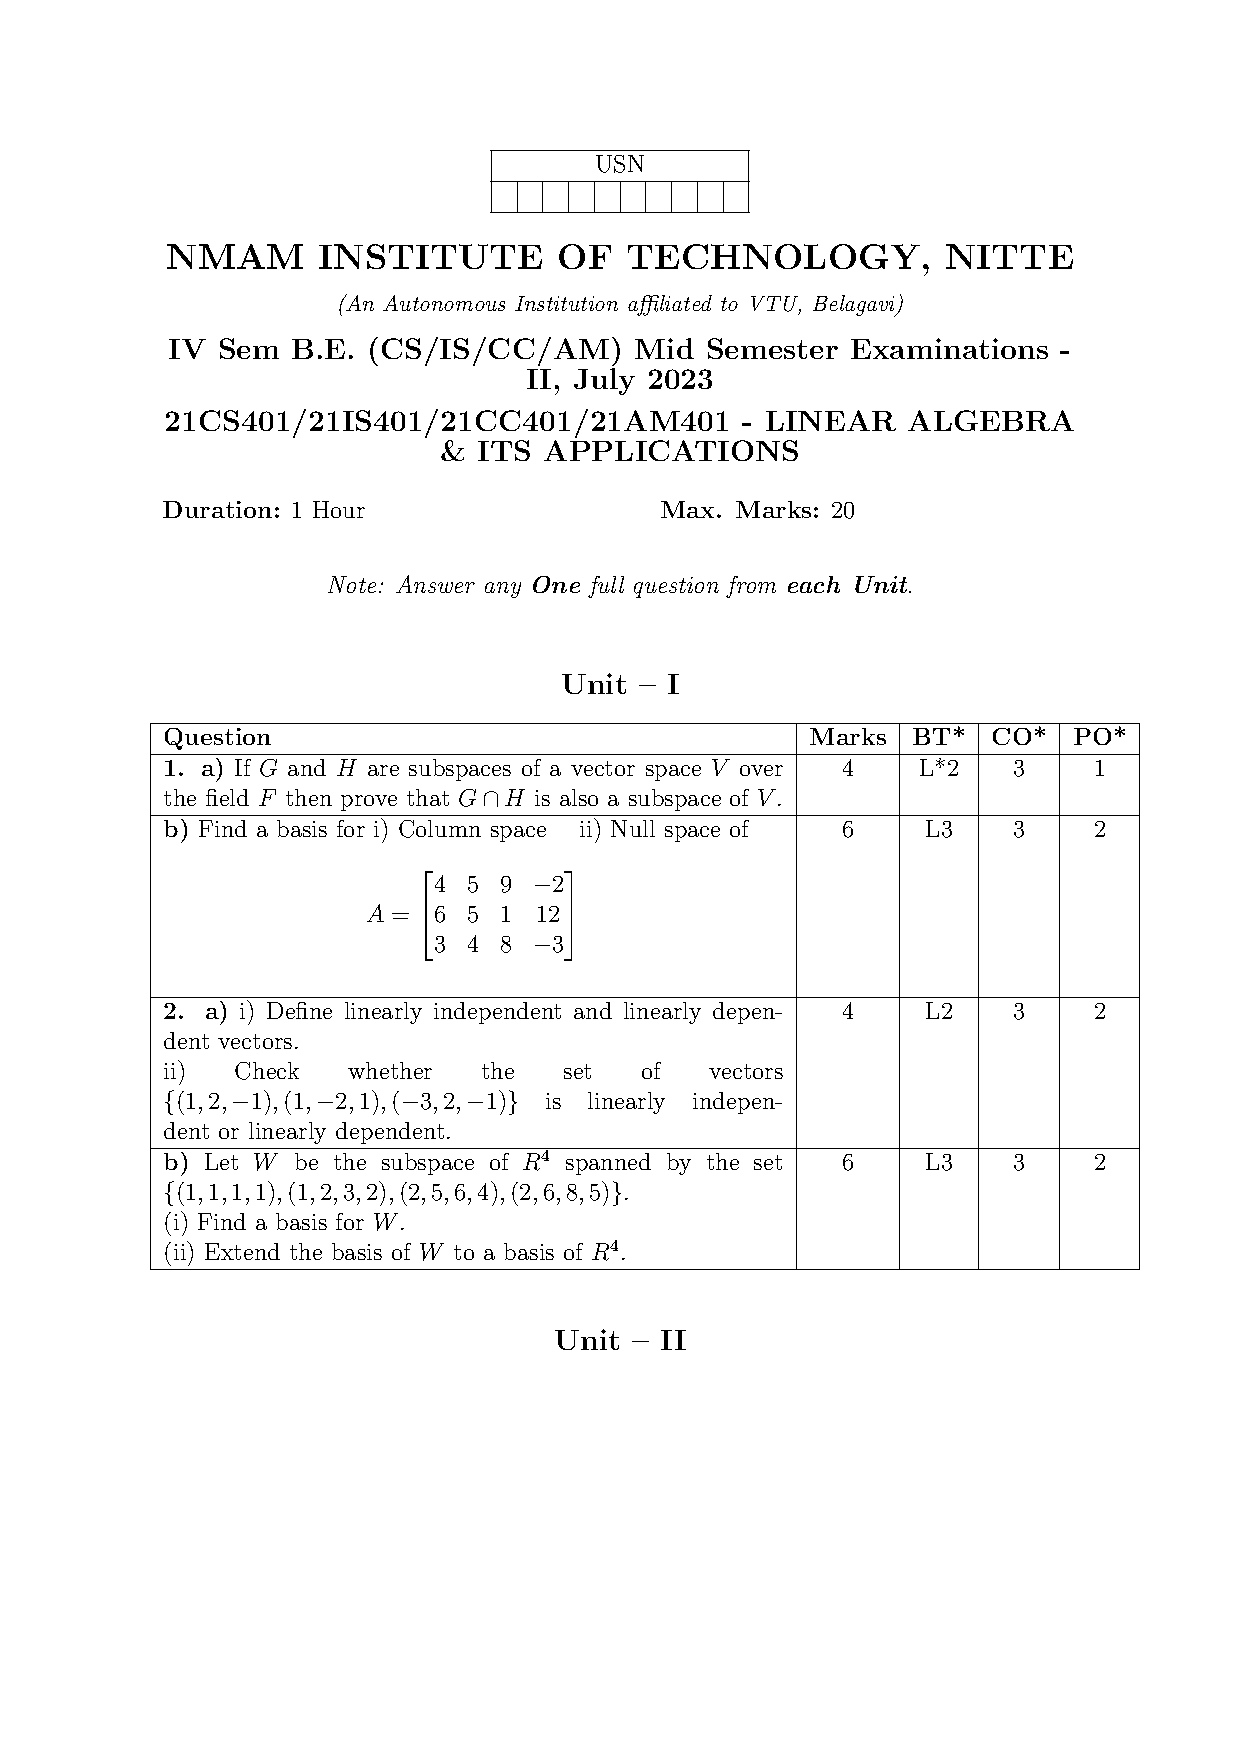
\includepdf[pages=-]{paper1_linear_algebra_july2023.pdf}
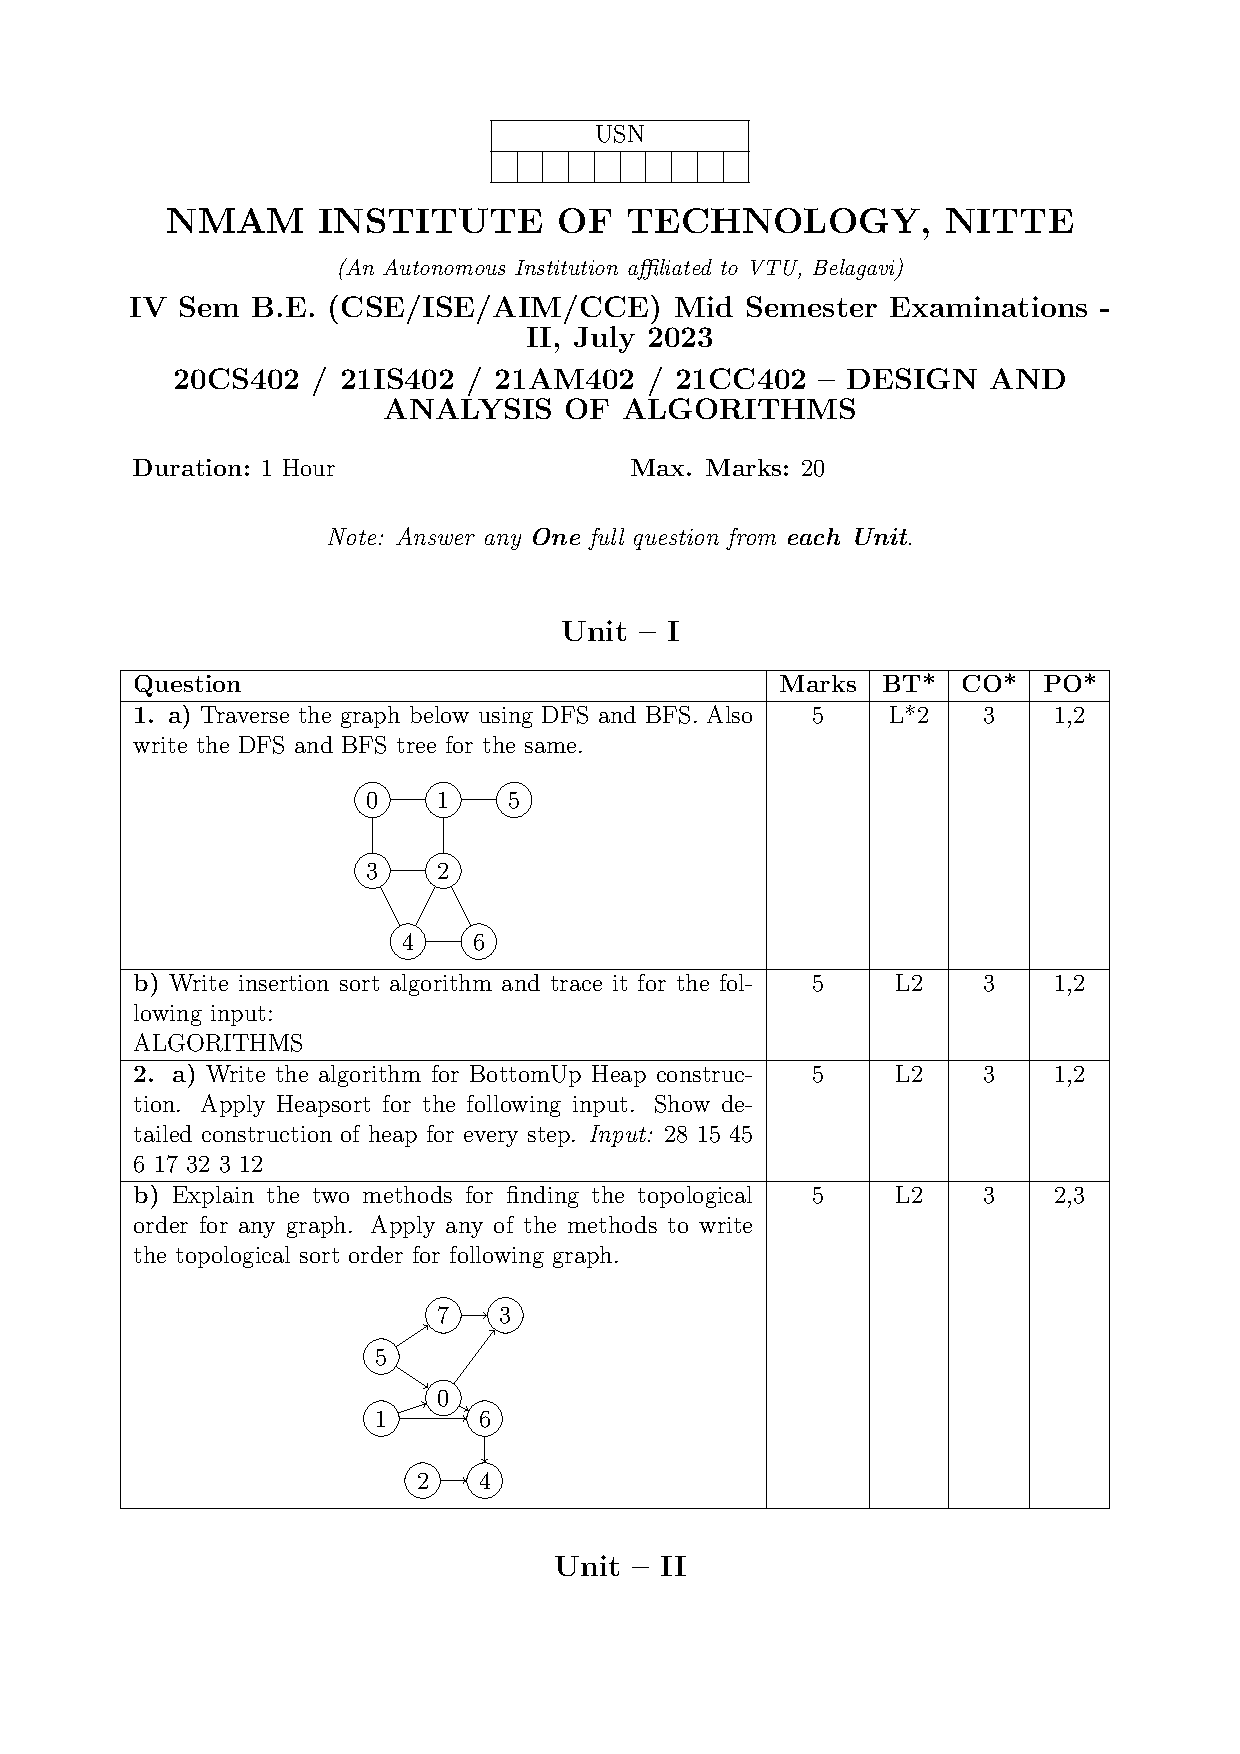
\includepdf[pages=-]{paper2_daa_july2023.pdf}
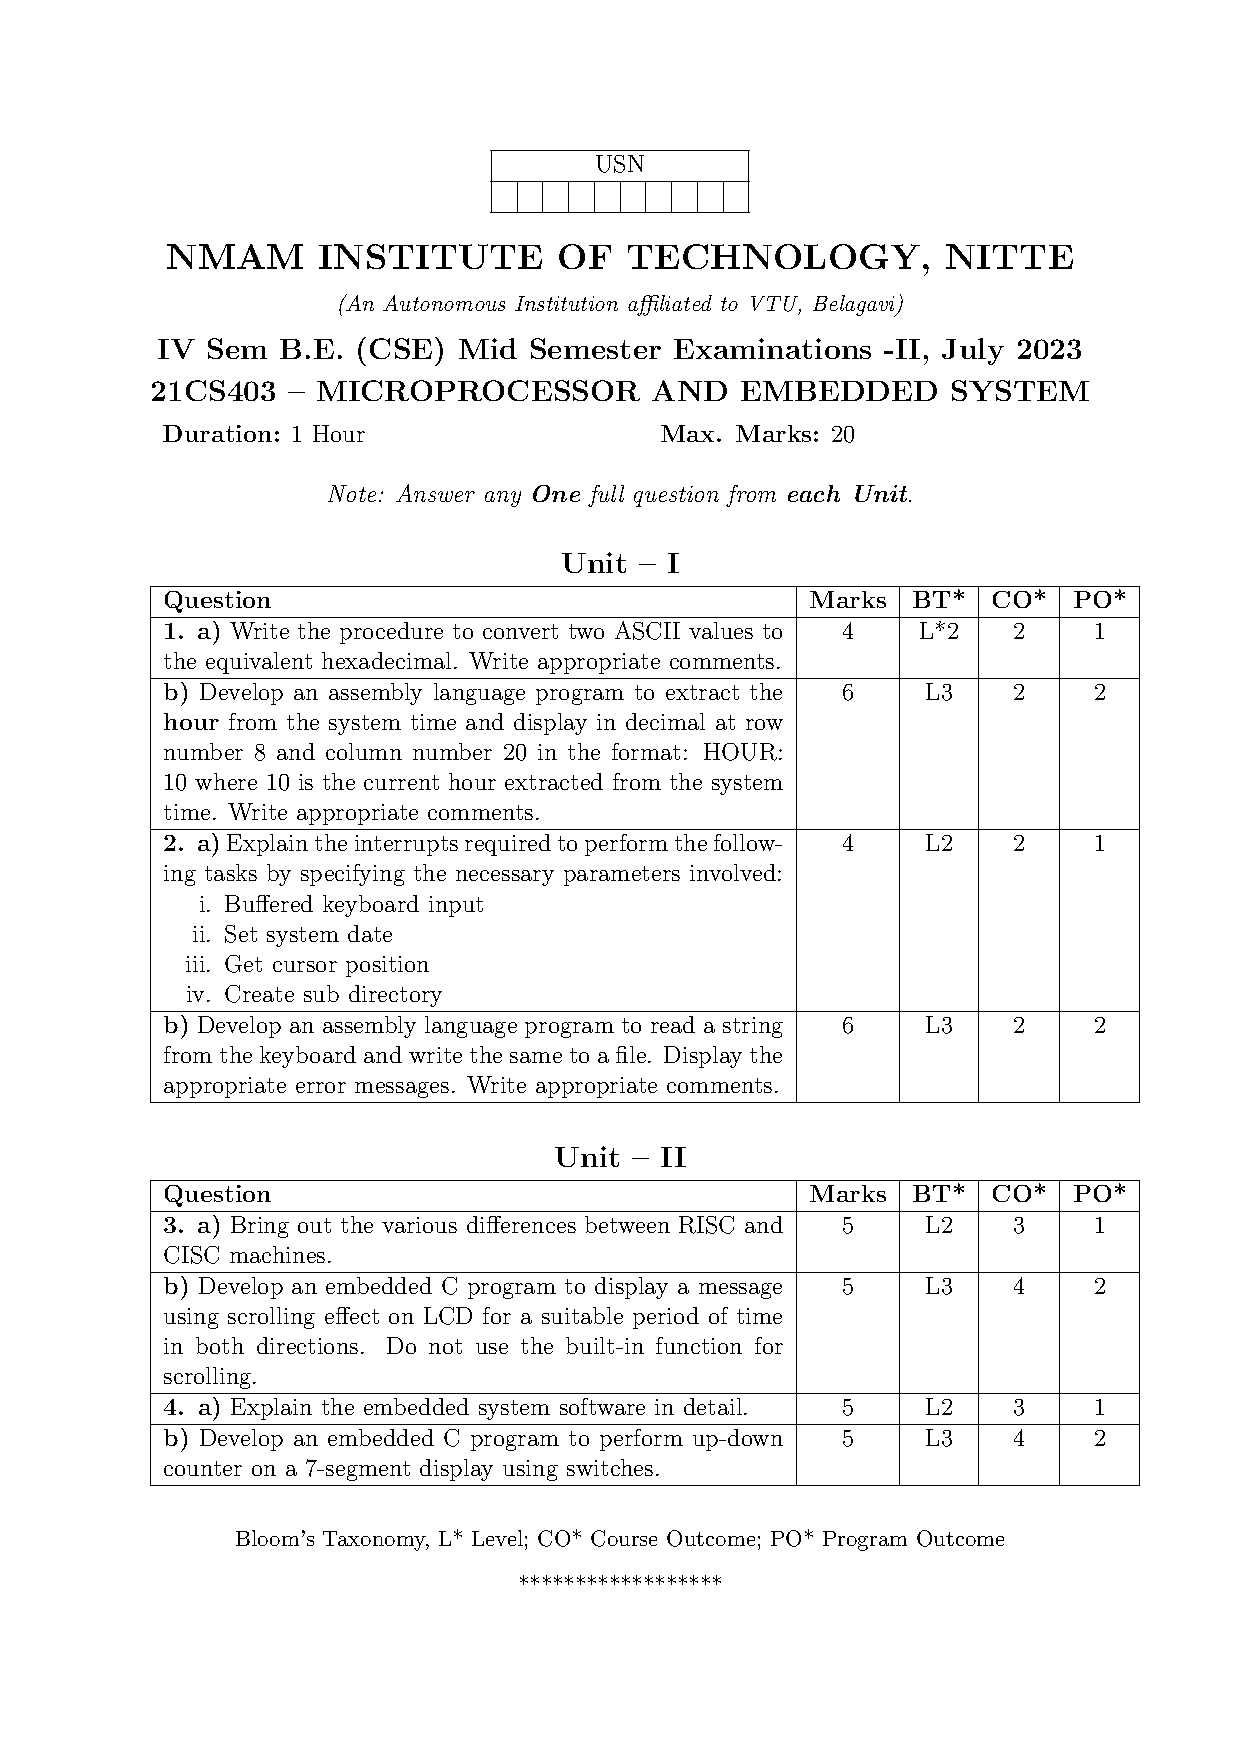
\includepdf[pages=-]{paper3_microprocessor_july2023.pdf}
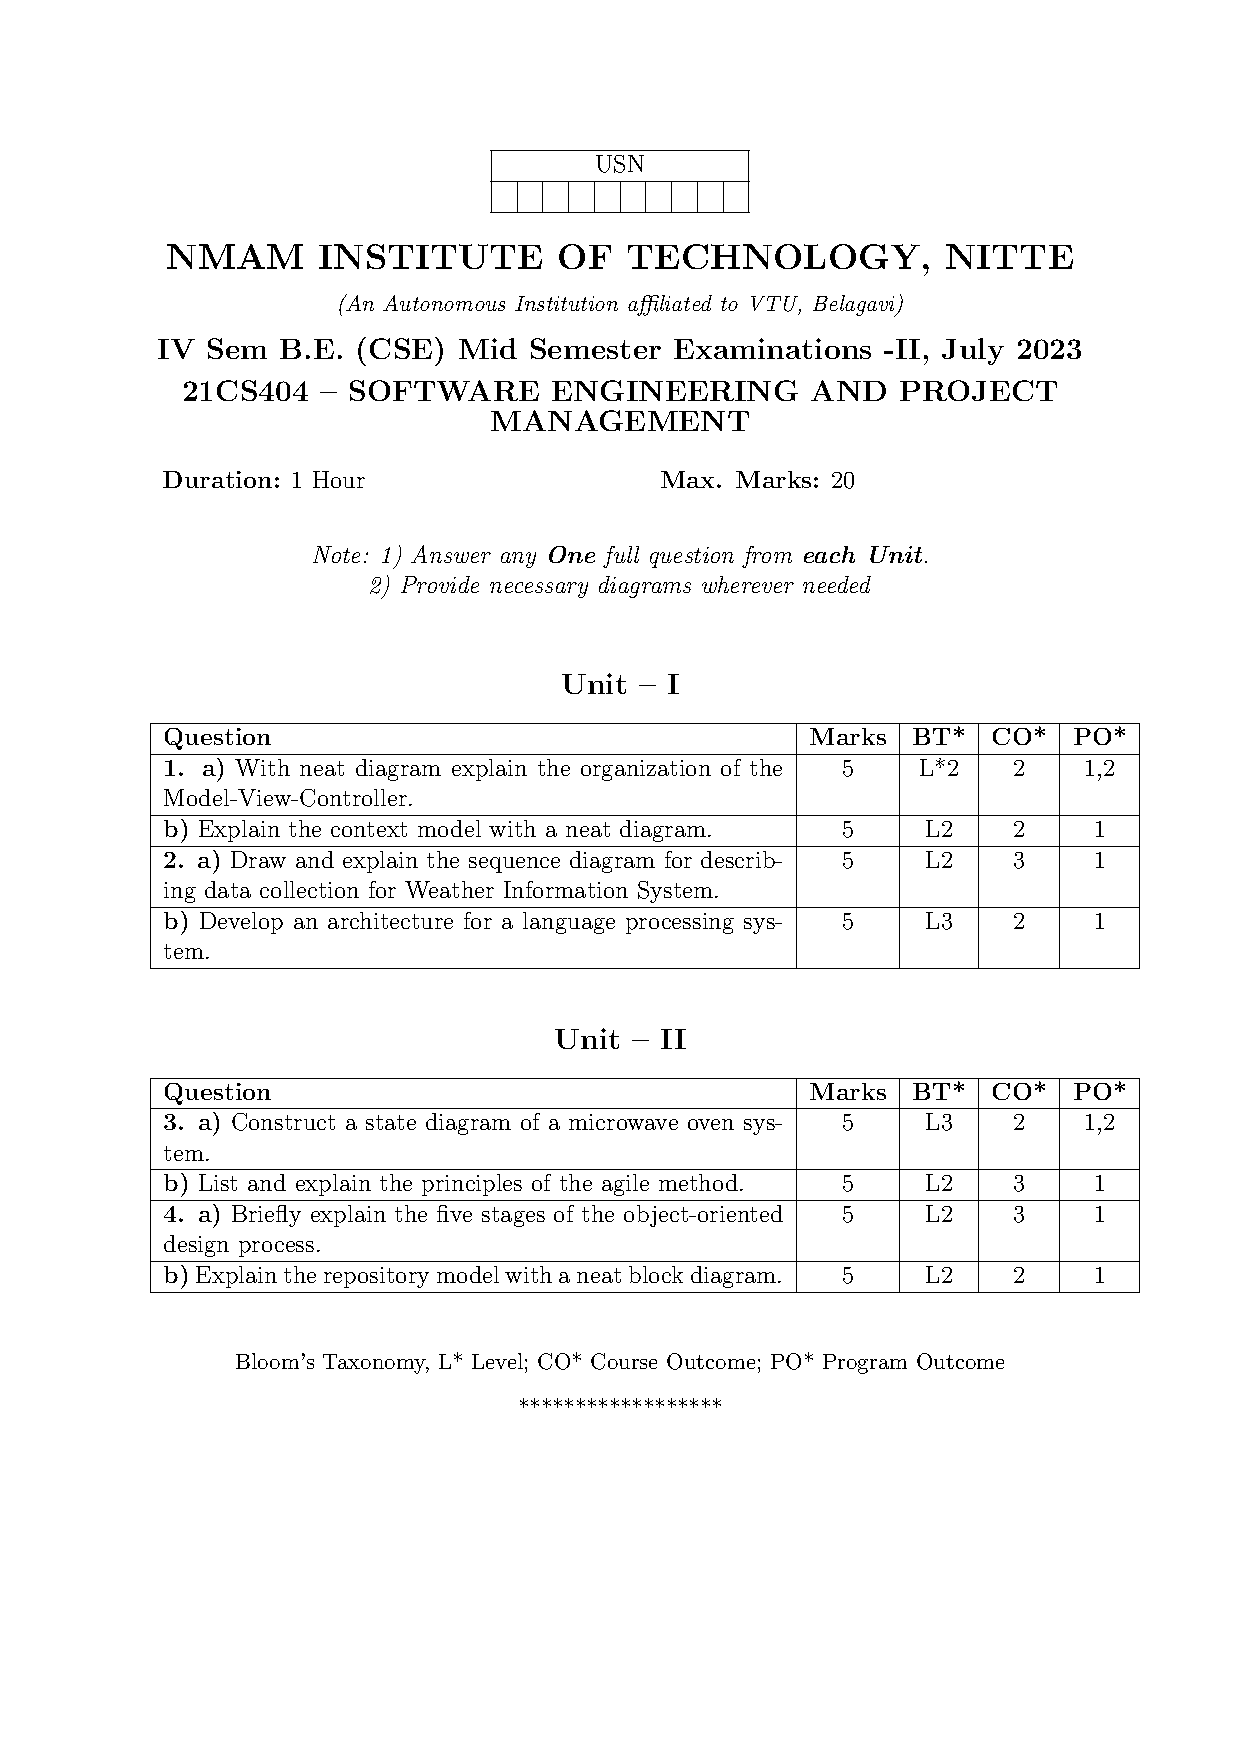
\includepdf[pages=-]{paper4_sepm_july2023.pdf}
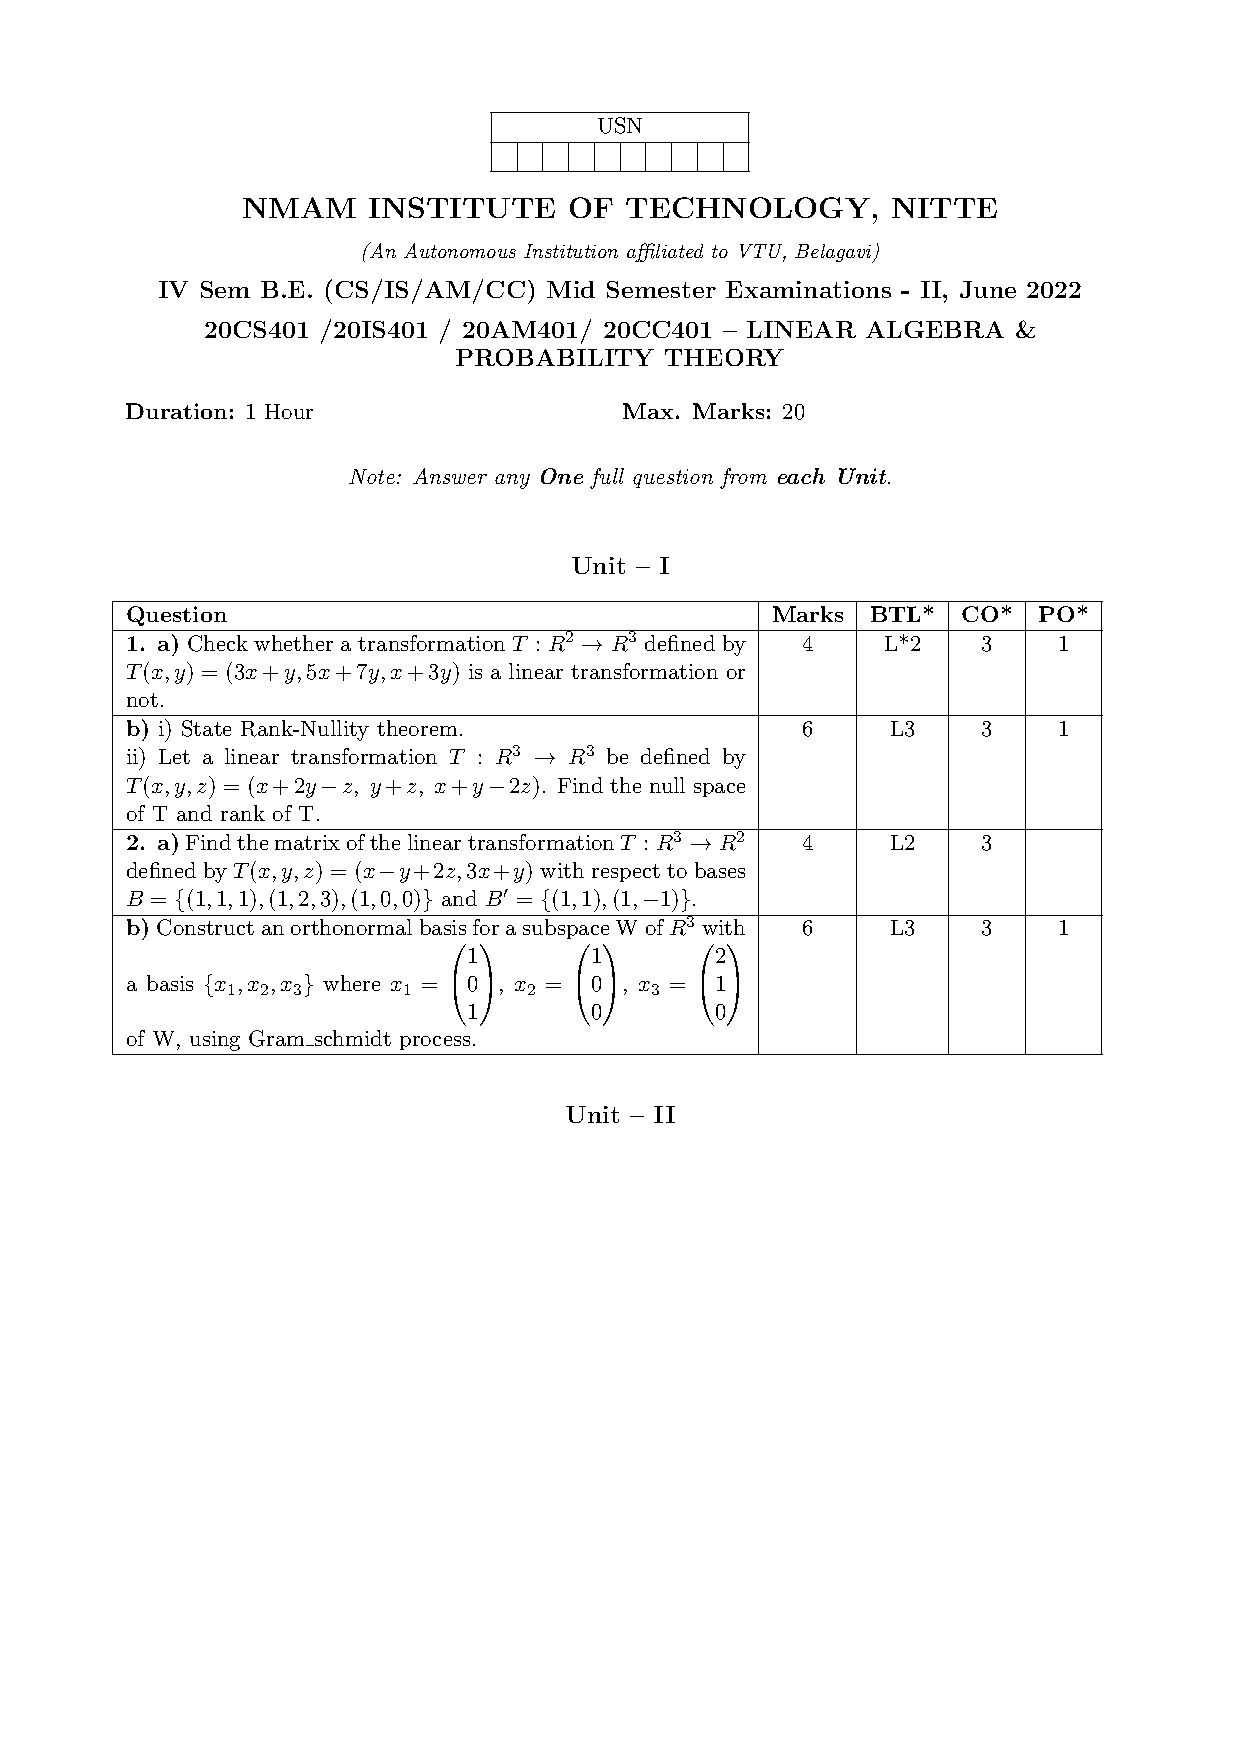
\includepdf[pages=-]{paper5_linear_algebra_prob_june2022.pdf}
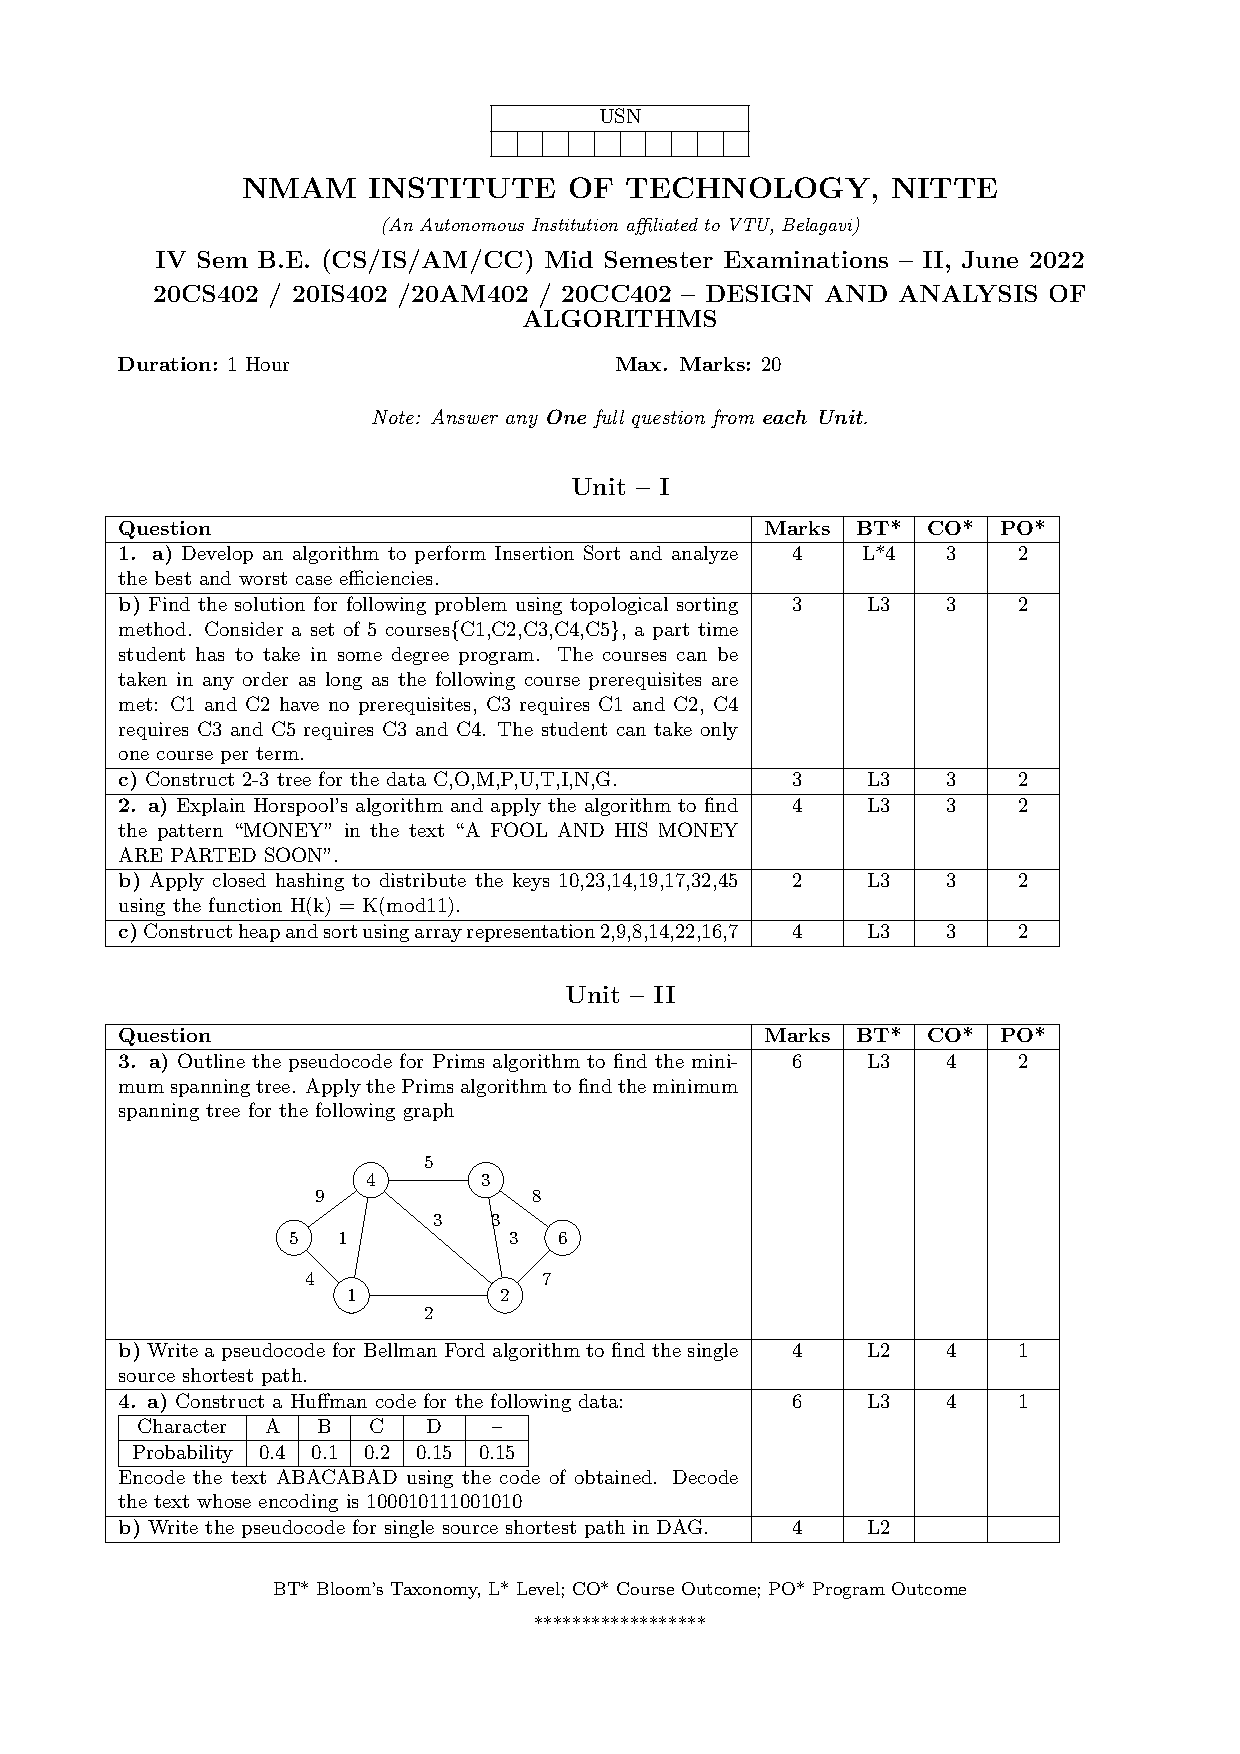
\includepdf[pages=-]{paper6_daa_june2022.pdf}

\end{document}
